\chapter{Reinforcement Learning Path Tracing}
\label{chapter RL}
Traditional path-tracing struggles for scenes where indirect lighting dominates. To alleviate this problem, this project implements a variant of path-tracing described at \cite{RLPT}, where reinforcement learning guides the generation of new rays.

\section{Motivation}
As described in section \ref{subsection MIS}, the path-tracing integrator samples from two MIS distributions: $p_{ref}$ which matches the local reflectance, and $p_{rad}$ which only samples points on light sources. The efficiency of this method relies on the assumption that one of $p_{ref}$ and $p_{rad}$ is a good match for the integrand of equation \ref{rendering equation with cast}. However, this is not always true, as exemplified by the scene rendered below.

\begin{figure}[H]
    \centering
    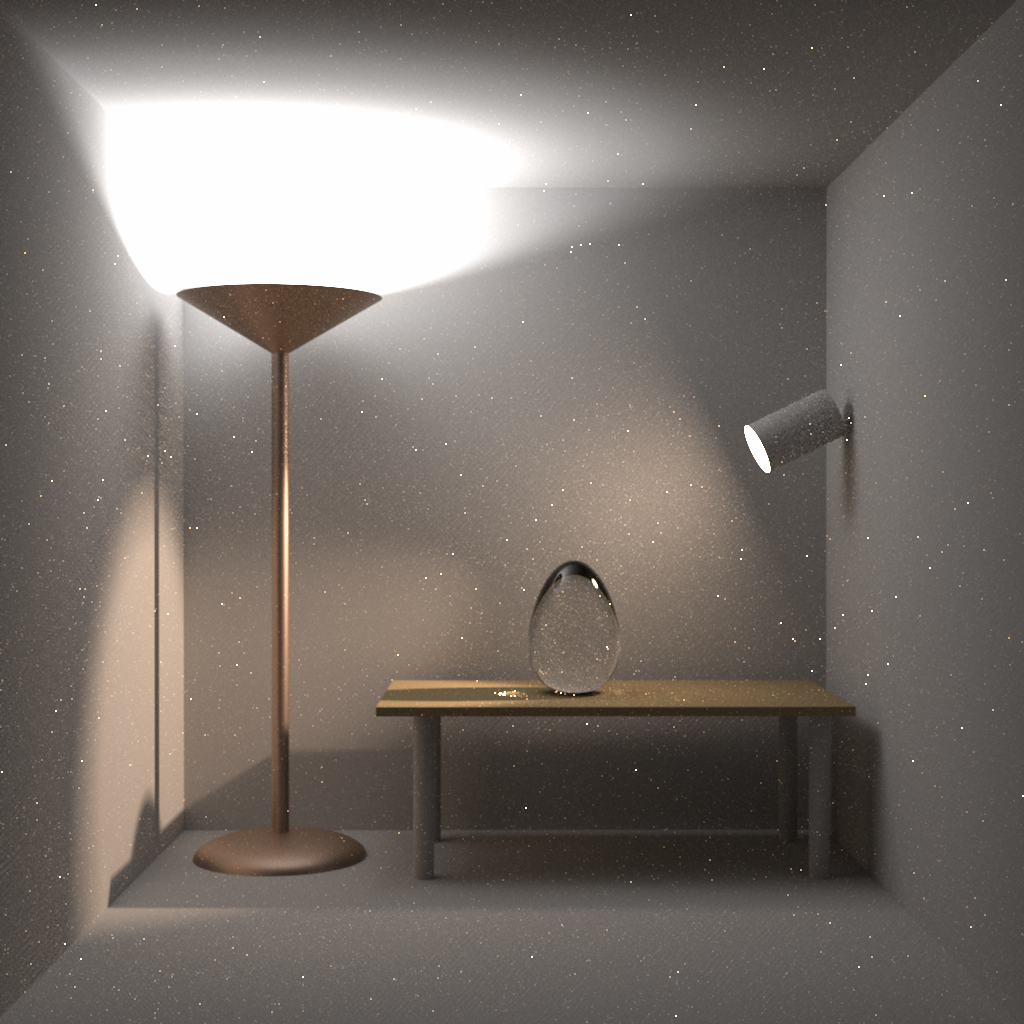
\includegraphics[height=6.1cm]{veach-bidir2_1024spp_rlpath.png}
\end{figure}

In this scene, both light sources are surrounded by opaque geometries, which means only a small region can be illuminated directly. Furthermore, the reflected radiance from this small region is the primary source of illumination for most surfaces in the scene. During path-tracing, the light sources sampled from $p_{rad}$ are often occluded, and hence $p_{rad}$ is poor match for the integrand. The directions sampled from $p_{ref}$ are also rarely useful, because only a small set of directions provides illumination. As both MIS distribution are ineffective, the algorithm converges extremely slowly.

\section{Method}
This projects implements the algorithm proposed by \cite{RLPT}, which uses online reinforcement learning to identify a distribution $p_{RL}$ of rays that is a good match for the integrand of the rendering equation.

In the reinforcement learning setting, an agent, starting from state $S_1$, interacts with an environment through a sequence of actions $A_1,A_2,...,A_N$. After each action $A_t$, the agent receives a reward $R_{t+1}$, and transitions into a new state $S_{t+1}$. Often, the goal of the agent is to maximize the rewards it receives through the actions. The following figure illustrates this system.

\begin{figure}[H]
    \centering
    


\tikzset{every picture/.style={line width=0.75pt}} %set default line width to 0.75pt        

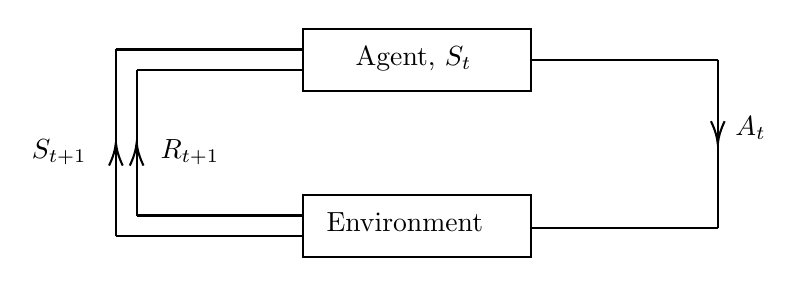
\begin{tikzpicture}[x=0.75pt,y=0.75pt,yscale=-1,xscale=1]
%uncomment if require: \path (0,300); %set diagram left start at 0, and has height of 300

%Shape: Rectangle [id:dp2545614332428212] 
\draw   (260,50) -- (370,50) -- (370,80) -- (260,80) -- cycle ;
%Shape: Rectangle [id:dp763438501832852] 
\draw   (260,130) -- (370,130) -- (370,160) -- (260,160) -- cycle ;
%Straight Lines [id:da1130501361879439] 
\draw    (370,65) -- (460,65) ;
%Straight Lines [id:da8576123899691459] 
\draw    (460,65) -- (460,146) ;
\draw [shift={(460,105.5)}, rotate = 270] [color={rgb, 255:red, 0; green, 0; blue, 0 }  ][line width=0.75]    (10.93,-3.29) .. controls (6.95,-1.4) and (3.31,-0.3) .. (0,0) .. controls (3.31,0.3) and (6.95,1.4) .. (10.93,3.29)   ;
%Straight Lines [id:da911132387231417] 
\draw    (460,146) -- (370,146) ;
%Straight Lines [id:da8508282995270846] 
\draw    (170,150) -- (260,150) ;
%Straight Lines [id:da6694647184777693] 
\draw    (170,150) -- (170,60) ;
\draw [shift={(170,105)}, rotate = 450] [color={rgb, 255:red, 0; green, 0; blue, 0 }  ][line width=0.75]    (10.93,-3.29) .. controls (6.95,-1.4) and (3.31,-0.3) .. (0,0) .. controls (3.31,0.3) and (6.95,1.4) .. (10.93,3.29)   ;
%Straight Lines [id:da6660171198842968] 
\draw    (260,60) -- (170,60) ;
%Straight Lines [id:da5838360811210379] 
\draw    (180,140) -- (260,140) ;
%Straight Lines [id:da6257626222476109] 
\draw    (180,140) -- (180,70) ;
\draw [shift={(180,105)}, rotate = 450] [color={rgb, 255:red, 0; green, 0; blue, 0 }  ][line width=0.75]    (10.93,-3.29) .. controls (6.95,-1.4) and (3.31,-0.3) .. (0,0) .. controls (3.31,0.3) and (6.95,1.4) .. (10.93,3.29)   ;
%Straight Lines [id:da8200304450497333] 
\draw    (260,70) -- (180,70) ;

% Text Node
\draw (284,57) node [anchor=north west][inner sep=0.75pt]   [align=left] {Agent, $\displaystyle S_{t}$};
% Text Node
\draw (270,137) node [anchor=north west][inner sep=0.75pt]   [align=left] {Environment};
% Text Node
\draw (467,91) node [anchor=north west][inner sep=0.75pt]   [align=left] {$\displaystyle A_{t}$};
% Text Node
\draw (128,102) node [anchor=north west][inner sep=0.75pt]   [align=left] {$\displaystyle S_{t+1}$};
% Text Node
\draw (190,102) node [anchor=north west][inner sep=0.75pt]   [align=left] {$\displaystyle R_{t+1}$};


\end{tikzpicture}

\end{figure}

A commonly used method to guide an agent is to maintain a table $Q$, where the $Q(s,a)$ is an indication of how good is the choice of taking the action $a$ at state $s$. A well-known method for updating $Q$ and moving the agent at the same time is the \textit{Expected Sarsa} strategy. At each state $s$, the strategy chooses an action $a$ from a distribution $\pi(s,a)$ which depends on $Q(s,a)$. This gives the agent a reward $R(s,a)$, and leads the agent to a new state $S'$. The algorithm then updates $Q(s,a)$ by the following formula:
\begin{align*}
    Q(s,a) := (1-\alpha) Q(s,a) + \alpha  \left(R(s,a)+\gamma \sum_{a'} \pi(s',a')Q(s',a') \right)
\end{align*}
where $\alpha\in [0,1]$ is a learning rate, and $\gamma\in [0,1]$ a discount factor which reflects the fact that future awards are less important than immediate ones. Intuitively, this algorithm attempts to balance the \textit{exploitation} of actions with high $Q$ values and the \textit{exploration} of actions with low $Q$ values.

Path-tracing bears many similarities with expected Sarsa. Specifically,
\begin{itemize}
    \item Each surface point $p$ can be regarded as a state $s$.
    \item The incoming direction $\omega_i$ to be traced can be seen as the action taken $a$.
    \item The actively emitted radiance $L_e$ received by $p$ from $\omega_i$ can be viewed as the immediate reward $R(a,s)$.
    \item The reflectance term $f_r(p,\omega_o,\omega_i)\cos \theta_i$ corresponds to the discount factor $\gamma$.
    \item The incoming radiance $L_i$ corresponds to $Q$.
\end{itemize}
In \cite{RLPT}, it was proposed that the expected Sarsa algorithm can be used learn the distribution of $Q$ (as thus $L_i$). When weighted (discounted) by the reflectance term $f_r(p,\omega_o,\omega_i)\cos \theta_i$, this distribution becomes a good distribution to sample incoming rays from, according to importance sampling.

Implementation-wise, notice that the domain of states $S$ and actions $A$ are both continuous, which makes a tabulated representation of $Q$ impossible. To work around this, this project divides the entire scene into a 3D grid, typically of size $32\times 32\times 32$. All surface points within the same grid cell are considered to be at the same state $s$. Moreover, at each grid cell, the spherical domain of incoming directions $\omega_i$ is also divided into 128 equally-sized sectors, and the directions in each sector are mapped to the same action $a$. 

During path-tracing, at each surface point $p_n$, instead of sampling a direction from the reflectance-matching $p_{ref}$, the algorithm uses the following sampling procedure:

\begin{algorithm}[H]
    \label{algo sample from Q}
    Finds the grid cell $s_n$ that encloses $p_n$\;
    \ForEach{\upshape sector $a$ at the cell $s_n$}{
        Sample a direction $\omega_i$ within $k$ uniformly at random\;
        Compute the discounted $Q$ value $Q'(s_n,a):= f_r(p,\omega_o,\omega_i)\cos \theta_i Q(s_n,a)$\;
    }
    Construct the discrete distribution over sectors $p_{sec,n}(a)=\frac{Q'(s_n,a)}{\sum_{a'}Q'(s_n,a')}$\;
    Sample a sector $a_n$ from $p_{sec,n}$\;
    Sample a direction $\omega_i$ within $a_n$ to trace the next ray towards\;
    \caption{Reinforcement Learning Guided Ray Generation}
\end{algorithm} 

~

After tracing $\omega_i$ from $p_n$ to find the next surface point $p_{n+1}$, the algorithm uses expected Sarsa to update the $Q$ table:
\begin{align*}
    Q(s,a) := (1-\alpha) Q(s,a) + \alpha  \left(L_e(p_{n+1}\to p_n)+ \sum_{a'} p_{sec,n+1}(a')  Q'(s_{n+1},a')\right)
\end{align*}

To illustrate the benefit brought by reinforcement learning, the following figure compares the same scene rendered by traditional path tracing and with reinforcement learning guided path tracing. Both images are rendered with 64 samples per pixel, and the difference between them is blatant. 

\begin{figure}[H]
    \centering
    
    \begin{minipage}[t]{.99\textwidth}
        \centering
        \vspace{0pt}
        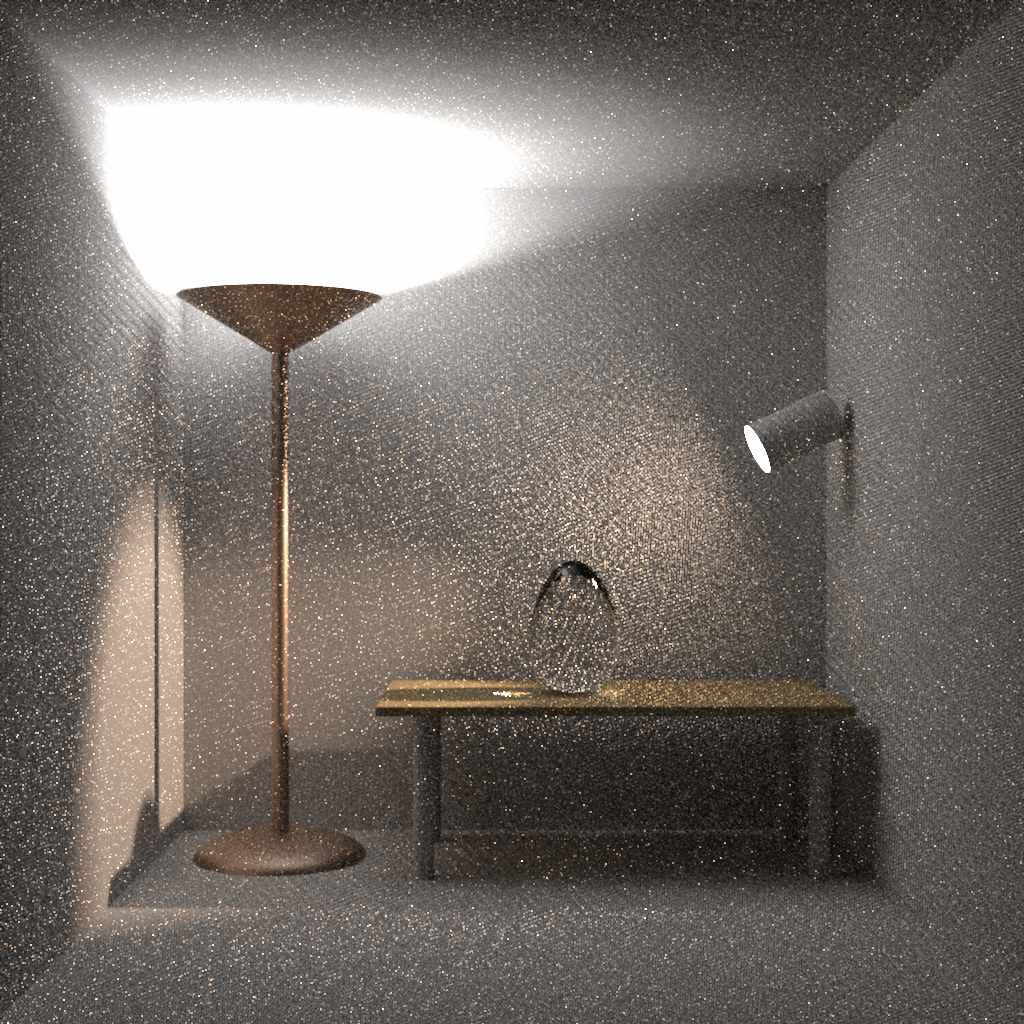
\includegraphics[width=.68\textwidth]{veach-bidir2_64spp_path.png}
        \subcaption{Traditional path tracing}
    \end{minipage}
    
    \vspace{0.3cm}

    \begin{minipage}[t]{.99\textwidth}
        \centering
        \vspace{0pt}
        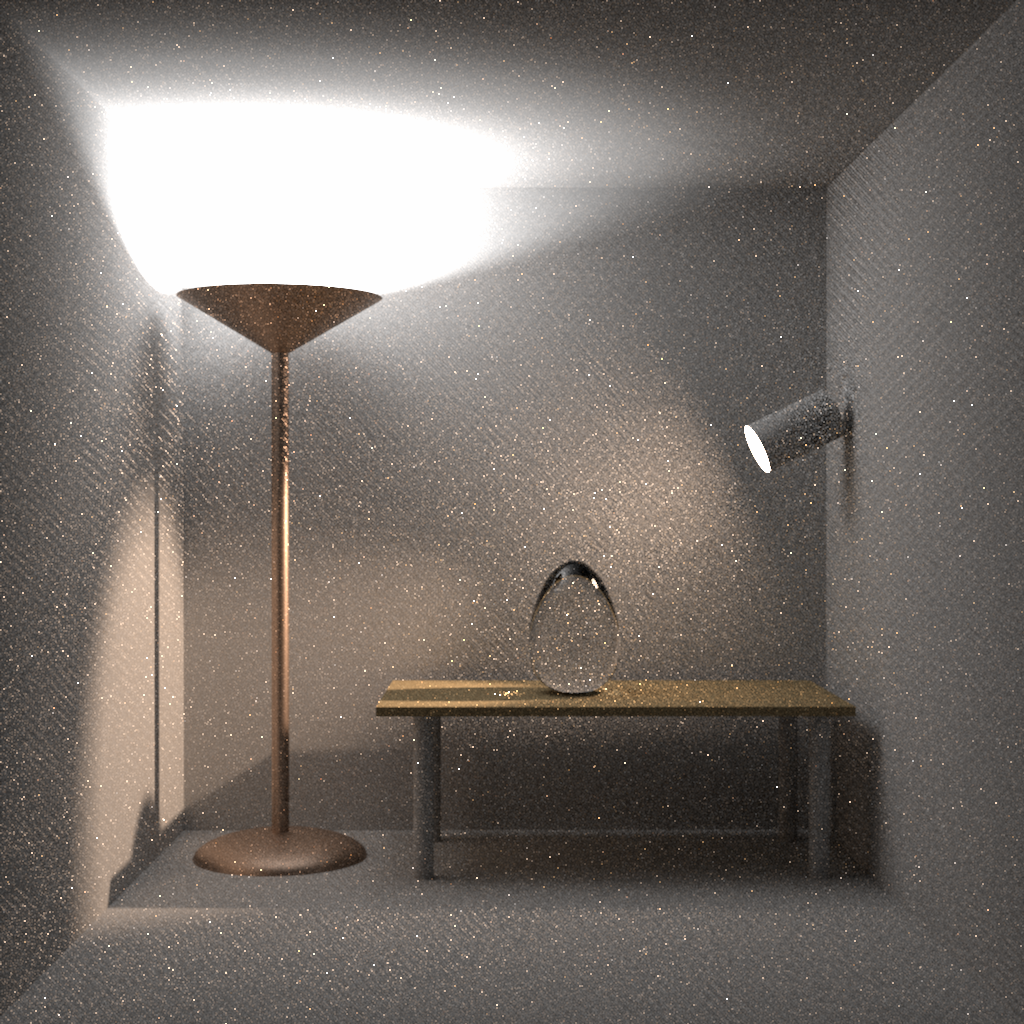
\includegraphics[width=.68\textwidth]{veach-bidir2_64spp_rlpath.png}
        \subcaption{Reinforcement learning path tracing}
    \end{minipage}
    
    \caption{Impacts of reinforcement learning}
    \label{fig RL comparison}
\end{figure}